\newcommand\user[2]{
	\begin{scope}[xshift=#1cm, yshift=#2cm]
		\clip (0, 0) circle (0.5);
		\fill[black] (0, 0) circle (0.5);
		\fill[white] (0, 0) circle (0.48);
		\fill[black] (0, -0.675) circle (0.4);
		\fill[black] (0, 0.075) circle (0.24);
	\end{scope}
}

\newcommand\ip[2]{
	\begin{scope}[xshift=#1cm, yshift=#2cm]
		%\rectangle[fill=black, rounded corners=0.2cm] (-0.5, -0.7) -- (0.5, 0.7);
		\draw[fill=black, thick, rounded corners=0.15cm] (-0.3, -0.5) rectangle (0.3, 0.5);
		\draw[fill=white] (0, -0.3) circle (0.1);
		\draw[fill=white, rounded corners=0.07cm] (-0.2, -0.1) rectangle (0.2, 0.0);
		\draw[fill=white, rounded corners=0.07cm] (-0.2, 0.1) rectangle (0.2, 0.2);
		\draw[fill=white, rounded corners=0.07cm] (-0.2, 0.3) rectangle (0.2, 0.4);
	\end{scope}
}

\newcommand\www[2]{
	\begin{scope}[xshift=#1cm, yshift=#2cm]
		\clip (0, 0) circle (0.5);
		\fill[yellow!65!black] (0, 0) circle (0.5);
		\fill[white] (-0.5, -0.175) rectangle (0.5,0.175);
		\node[text=yellow!65!black] at (0,0) {www};
	\end{scope}
}

\newcommand\malwww[2]{
	\begin{scope}[xshift=#1cm, yshift=#2cm]
		\clip (0, 0) circle (0.5);
		\fill[red!65!black] (0, 0) circle (0.5);
		\fill[white] (-0.5, -0.175) rectangle (0.5,0.175);
		\node[text=yellow!65!black] at (0,0) {www};
	\end{scope}
}

\newcommand\wwwline[3]{
	\node[circle, minimum size=1.1cm] (#3) at (0, #1) {};
	\www{0}{#1}
	\node[text width=50mm, align=right] at (-5, #1) {#2};
}

\newcommand\malwwwline[3]{
	\node[circle, minimum size=1.1cm] (#3) at (0, #1) {};
	\malwww{0}{#1}
	\node[text width=50mm, align=right] at (-5, #1) {#2};
}

\newcommand\userline[2]{
	\node[circle, minimum size=1.1cm] (#2) at (5, #1) {};
	\user{5}{#1}
	\node[text width=50mm, align=left] at (10, #1) {#2};
}

\newcommand\ipline[3]{
	\node[circle, minimum size=1.1cm] (#3) at (5, #1) {};
	\ip{5}{#1}
	\node[text width=50mm, align=left] at (10, #1) {#2};
}

\scalebox{0.5}{

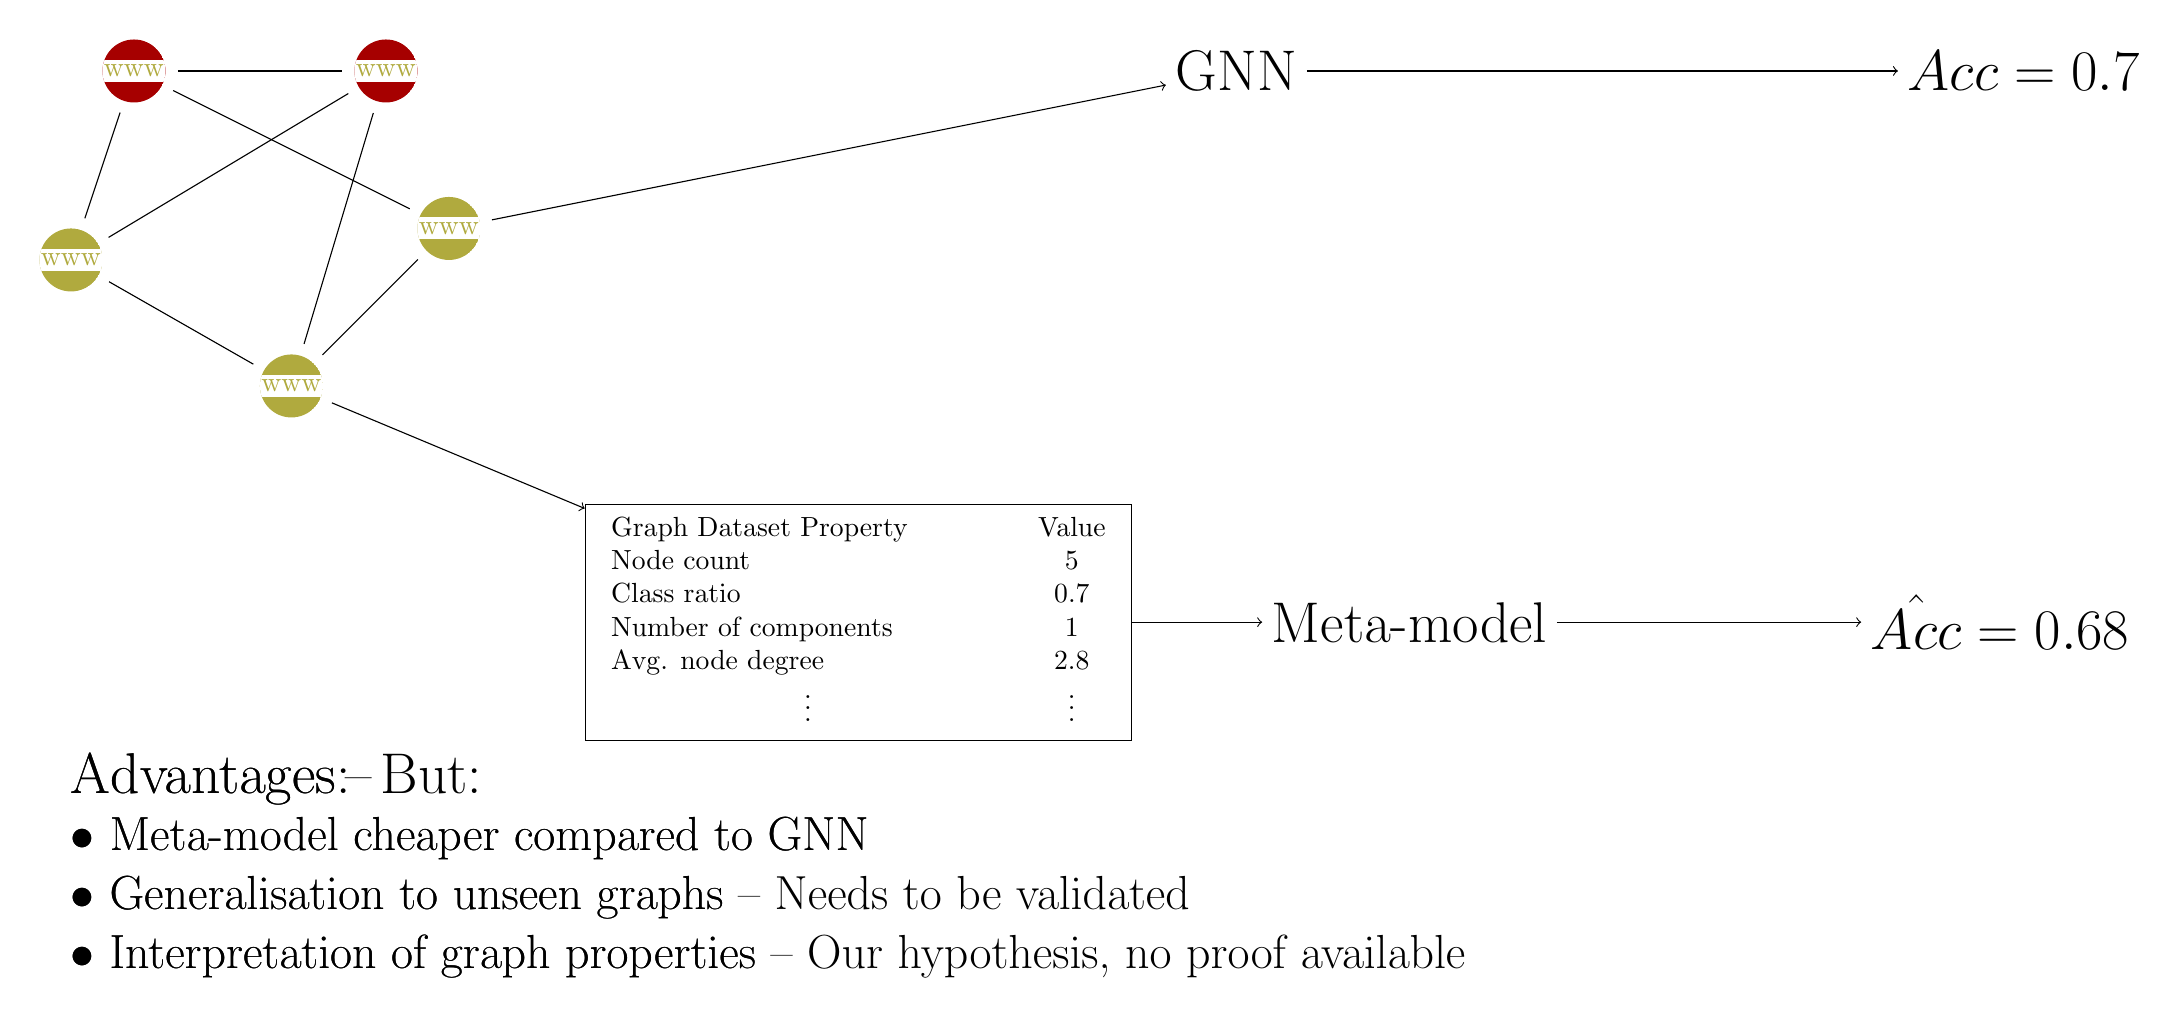
\begin{tikzpicture}

\begin{scope}[scale=0.8, xshift=-12cm, yshift=7cm]  
\node[circle, minimum size=1.1cm] (d1) at (-2, 3) {};
\malwww{-2}{3}	
\node[circle, minimum size=1.1cm] (d2) at (2, 3) {};
\malwww{2}{3}	
\node[circle, minimum size=1.1cm] (d3) at (-3, 0) {};
\www{-3}{0}
\node[circle, minimum size=1.1cm] (d4) at (3, 0.5) {};
\www{3}{0.5}	
\node[circle, minimum size=1.1cm] (d5) at (0.5, -2) {};
\www{0.5}{-2}
\draw (d1) -- (d2);
\draw (d1) -- (d3);
\draw (d1) -- (d4);
\draw (d2) -- (d3);
\draw (d2) -- (d5);
\draw (d3) -- (d5);
\draw (d4) -- (d5);
\end{scope}

\node[font=\huge] (m) at ([xshift=10cm, yshift=2cm] d4.center) {GNN};

\node[font=\huge] (p) at ([xshift=10cm] m.center) {$Acc=0.7$};

\draw[->] (d4)--(m);
\draw[->] (m)--(p);

\uncover<2->{
\node [draw] (r) at (-2, 1) {
    \begin{tabular}{p{5cm}c}
        Graph Dataset Property & Value  \\
        \midrule
        Node count             & 5      \\
        Class ratio            & 0.7    \\
        Number of components   & 1      \\
        Avg. node degree       & 2.8    \\
        \centerline{\vdots}    & \vdots \\
    \end{tabular}
};
\draw[->] (d5) -- (r);
\node[font=\huge] at (5,1) (mm) {Meta-model};
\draw[->] (r) -- (mm);
\node[font=\huge] at (12.5,1) (pm) {$\hat{Acc} = 0.68$};
\draw[->] (mm) -- (pm);
}


\uncover<3>{
    \node[text width=110mm, align=left] at (-6.5, -1) {
{\huge{Advantages:}}
};
    \node [font=\LARGE, text width=110mm, align=left] (top)    at (-6.5,-1.75) {$\bullet$ Meta-model cheaper compared to GNN};
    \node [font=\LARGE, text width=110mm, align=left] (middle) at (-6.5,-2.5)  {$\bullet$ Generalisation to unseen graphs};
    \node [font=\LARGE, text width=110mm, align=left] (bottom) at (-6.5,-3.25)  {$\bullet$ Interpretation of graph properties};
}

\uncover<4>{
    \node[text width=180mm, align=left] at (-3, -1) {
{\huge{Advantages -- \alert{But}:}}
};
    \node [font=\LARGE, text width=180mm, align=left] (top)    at (-3,-1.75) {$\bullet$ Meta-model cheaper compared to GNN};
    \node [font=\LARGE, text width=180mm, align=left] (middle) at (-3,-2.5)  {$\bullet$ Generalisation to unseen graphs -- \alert{Needs to be validated}};
    \node [font=\LARGE, text width=180mm, align=left] (bottom) at (-3,-3.25)  {$\bullet$ Interpretation of graph properties -- \alert{Our hypothesis, no proof available}};
}
\end{tikzpicture}
}
